\subsection*{Santuario del Caos}
Cuando el grupo llega a los prados que limitan con el Bosque Oscuro, alcanzan a ver el intimidante Santuario del Caos a la distancia. A medida que se acercan, notan que la naturaleza se ha adueñado del santuario, pues sus paredes están dañadas y cubiertas de vegetación. Los cimientos del edificio han comenzado a sumergirse en el suelo. Una serenidad anormal rodea el santuario. No hay rastro de vida a la vista y la única entrada es un conjunto de escaleras quebradizas que bajan hacia la oscuridad. Después de bajar las escaleras, el grupo llega al sur del mapa que se muestra a continuación y apenas puede ver en la oscuridad. El sector norte está bloqueado por escombros provenientes de las columnas y del techo. Tras una inspección más cercana, el grupo se da cuenta de que este bloqueo no fue accidental, si no que alguien lo ha hecho a propósito.
\vspace{0.1cm}
\tcbox[left=1pt,top=1pt,right=1pt,bottom=1pt, boxsep=-1pt, colframe=accent, sharp corners]{
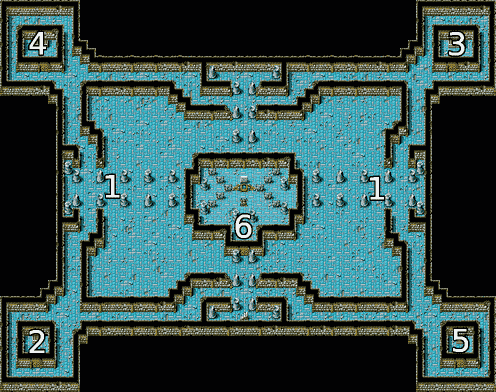
\includegraphics[width=0.98\columnwidth]{./art/maps/shrine.png}}

\subsubsection*{1 Trampas}
Ambas ubicaciones marcadas contienen una trampa mágica en el suelo que ha sido colocada por Garland para alertarlo e impedir que ingresen intrusos. Un personaje que esté activamente buscando trampas o que tome recaudos similares, notará la trampa mediante una tirada de DC 7. La trampa explota al pisarla e inflige 2d de daño de \hyperlink{type}{fuego }daños a todas las personas en un radio de 1u de su centro. \subsubsection*{2. Mímico}
Dentro de esta habitación hay un enorme cofre que al tocarlo se revela como un despiadado Mímico. Un personaje puede notar de antemano que hay algo extraño en el cofre pasando una tirada con DC 9. Si no tiene éxito, el Mímico obtiene automáticamente el mejor resultado posible en su tirada de iniciativa en la batalla.
\vfill
\monster{Mimic}{2}{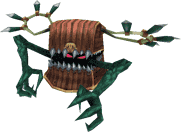
\includegraphics[width=0.25\textwidth]{./art/monsters/mimic.png}}
{
	HP: & \hfill 20 & MP: & \hfill 0\\
	STR: & \hfill 2 & DEF: & \hfill 0 \\
	MAG: & \hfill 0 & RES: & \hfill 0 \\
	AGI: & \hfill 2 & Size: & \hfill M\\
}
{
	\textbf{Bite}: 1d DMG \hfill \textbf{Drops:} 200 Gil	
}

\subsubsection*{3. Fuente de la sanación}
La pesada puerta de esta habitación está bloqueada y se puede destruir o forzar su cerradura pasando una tirada con DC de entre 6 y 9, dependiendo de la pericia del personaje. En esta habitación, el grupo encuentra un enorme cáliz que se encuentra en un pedestal de piedra lleno de lo que parece ser agua. Luego de una inspección más cercana, un personaje puede deducir que el líquido es de naturaleza mágica y que si alguien lo bebe, recupera por completo sus PV y PM inmediatamente. Sin embargo, el cáliz en sí no tiene propiedades mágicas y contiene solo 5 dosis del agua curativa. \subsubsection*{4. Cofres}
Esta sala contiene 2 cofres. Uno se puede abrir fácilmente y contiene 3 \hyperlink{item}{Pociones} y un \hyperlink{item}{Ala de Fénix}. El otro contiene el \textbf{Laúd de Sarah }y solo puede abrirse mediante una tirada con una DC que varía entre 7 y 10 según la pericia del personaje. También puede abrirse con una llave que Garland lleva consigo, pero el cofre es demasiado duro como para romper a la fuerza. \subsubsection*{5. Puerta secreta}
Esta sala está vacía, salvo por una gran lápida de piedra incrustada en la pared izquierda con varios símbolos diferentes. Después de una inspección más cercana, el grupo puede deducir que los símbolos describen una corta partitura de música. En la pared junto a ella hay una puerta secreta que se revela tocando la partitura con el Laúd de Sarah, y solo ella debería poder interpretar la melodía correctamente. La puerta secreta conduce a una pequeña sala con un pedestal de piedra que tiene el siguiente objeto: 
\vspace{0.3cm}
\accessory{Accesorios}{acc.png}{
 \hline Anillo \newline de Ángel & 2000 Gil & Si tienes este anillo equipado cuando caigas en estado \hyperlink{status}{KO}, puedes activar su efecto inmediatamente y volver a estar de pie con 1 PV. El anillo se destruye después de usar este efecto. \\
} 
%\pagebreak
\subsubsection*{6. Garland}
"Ahhh... los perritos falderos del rey. ¿Tienen idea de con quién se están metiendo?"
\indent -- Garland \\\\ 
En el centro del templo, el grupo finalmente se enfrenta a Garland. Sarah también está en esta habitación, encerrada en una jaula que se encuentra en una esquina. Garland es un hombre alto y fornido. Viste una armadura pesada y una capa morada y está armado con una espada. Es muy arrogante y cree que merece gobernar Cornelia porque es el guerrero más fuerte del reino. Desde que llegó, Garland ha estudiado los secretos oscuros del Santuario del Caos para aumentar su propio poder. Considera al grupo tan solo como una piedra más en el camino de sus grandes planes. \subsubsection*{Batalla final}
"¿Realmente creen que pueden enfrentarse a MÍ? De acuerdo…" \\
\indent -- Garland \\\\ 
Garland desenvaina su arma para comenzar la batalla y también invoca varios murciélagos para que lo asistan, uno por cada miembro del grupo. Durante la batalla, su posicionamiento se centra en arrinconar a los miembros del grupo individualmente mientras evita que lo superen en número. Prefiere que primero sus esbirros utilicen sus habilidades de larga distancia para luego intentar acabar con los enemigos que han sido debilitados. En la historia original, Garland utiliza un artefacto mágico para escapar después de ser derrotado y se convierte en el principal antagonista del juego. Si quieres continuar la aventura de forma diferente, también puede morir a mano de los aventureros o puedes dejar que los jugadores decidan su destino. Después de ser liberada de su prisión, Sarah sigue lógicamente muy asustada y traumada. Le agradece al grupo por rescatarla y les pide que encuentren su precioso laúd que Garland robó. El grupo puede rechazar su solicitud para regresar rápidamente a Cornelia. Sarah comprenderá pero no estará contenta.

\vfill
\monster{Murciélago}{1}{
\includegraphics[width=0.18\textwidth]{./art/monsters/bat.png}}
{
 PV: & \hfill 6 & PM: & \hfill 0\\
 FUE: & \hfill 0 & DEF: & \hfill 0 \\
 MAG: & \hfill 0 & RES: & \hfill 2 \\
 AGI: & \hfill 4 & Tamaño: & \hfill P\\
}
{
 \textbf{Dientes}: 1d de daño \hfill \textbf{Botín:} 100 Gil 
 
 \mpassive{Absorber}{Por cada \hyperlink{action}{Ataque} exitoso, recuperas 1d de PV.} 
}
\vfill
\monster{Garland}{3}{
\includegraphics[width=0.18\textwidth]{./art/monsters/garland.png}}
{
 PV: & \hfill 40 & PM: & \hfill 30\\
 FUE: & \hfill 3 & DEF: & \hfill 1 \\
 MAG: & \hfill 1 & RES: & \hfill 1 \\
 AGI: & \hfill 2 & Tamaño: & \hfill M\\
}
{
 \textbf{Espada Larga}: 1d de daño \hfill \textbf{Botín}: 1000 Gil, Llave 
 
 \mspell{Absorber}{8}{1t}{Único}{3u}{ Reduces 1d de los PV del objetivo y recuperas tus PV por el mismo valor.}{} \mspell{Silencio}{6}{1t}{Único}{3u}{El objetivo hace una tirada con DC 8. Si falla, sufre \hyperlink{status}{Silencio} por 3 turnos.}{\silence}
 \mreaction{Parada}{Cuando falles al intentar esquivar un \hyperlink{action}{Ataque}, Puedes hacer una tirada con DC~8. Si tienes éxito, el daño que recibes se reduce a la mitad.}
}
\vspace{2.2cm}
\pagebreak

\subsection*{Epílogo}
"¿Han... han venido a rescatarme? No sé cómo puedo darles las gracias..." \\ 
\indent -- Sarah \\\\ 
Después de rescatar a Sarah, el grupo debe regresarla sana y salva a Cornelia y, por lo tanto, tienen que volver a atravesar el largo camino que recorrieron para llegar al Santuario. El viaje debería ser en general tranquilo, pero si quieres puedes añadir algunas sorpresas. Sarah es una princesa joven con pelo turquesa como su madre y luce un vestido dorado y un colgante dorado adornado con joyas rojas. Es educada pero también muy tranquila y ausente: el secuestro ha dejado cicatrices físicas y mentales en ella. Sarah no es capaz de cuidar de sí misma, así que necesita ayuda y orientación de los aventureros durante el viaje. Durante el viaje, a menudo pregunta por Cornelia y su familia, mientras se culpa por todo lo que ha sucedido. 

\subsubsection*{Llegada}
"Gracias por traer a mi hija de nuevo a mi lado". \\ 
\indent -- Rey de Cornelia \\\\ 
Al entrar a Cornelia con la princesa, los aventureros son considerados héroes por los habitantes del pueblo y los guardias. En consecuencia, todas las personas del pueblo los reconocerán como tal. Los habitantes del castillo se sorprendieron al ver al grupo, ya que habían perdido toda esperanza de ver a la princesa de nuevo. El rey está muy agradecido con los aventureros y pide a sus servidores que preparen un banquete enorme en su honor esa misma noche. Al grupo se lo recompensa con una \textbf{Subida de nivel} por regresar a la princesa a casa. Además, el rey les ofrece enormes recompensas por rescatar a su hija como había prometido. En la historia original, el rey ordena a sus hombres que reconstruyan un antiguo puente destruido que conduce a otro gran continente para que los aventureros exploren. Dependiendo de cómo quieras continuar el juego, su regalo debería ser algo que ayude al grupo en sus próximas aventuras. Por ejemplo, podría obsequiarles un barco que les permita llegar a nuevos territorios o una casa en Cornelia si el pueblo sigue siendo de importancia. \subsubsection*{Conclusión}
Al rescatar a la princesa Sarah y derrotar a Garland, los aventureros han crecido como grupo y han desarrollado sus habilidades individuales. Aunque aún tienen mucho que aprender, han demostrado que son aventureros capaces de enfrentarse a los males presentes en mundo. Desde aquí, puedes continuar la aventura construyendo sobre el contenido que te presentamos aquí y creando tus propios lugares, personajes y desafíos. Antes de partir, el grupo puede decidir pasar un tiempo más en Cornelia para descansar y abastecerse de objetos y equipo.
